\documentclass{article}

\usepackage[margin=1.25in]{geometry}
\usepackage{graphicx}
\usepackage[hidelinks]{hyperref}
\usepackage{verbatimbox}
\usepackage{epigraph}

\setlength{\epigraphwidth}{0.6\textwidth}
\setlength{\parindent}{0pt}

\begin{document}

\title{Puzzle Prison Guide}
\date{}
\maketitle

\section*{Introduction}
This is a complete guide to the Amazon Alexa skill: Puzzle Prison. 
The game is set in a single room with five puzzles, the main two commands are \textit{walk to} and \textit{interact with}. 
To report bugs and give feedback on the game or this guide visit: \url{www.puzzleprison.uk}

\section*{Start}
When you start the game, the room is set up like diagram below.
To trigger the first letter you need to use the computer by saying \textit{interact with computer}.

\begin{figure}[htb]
	\centering
	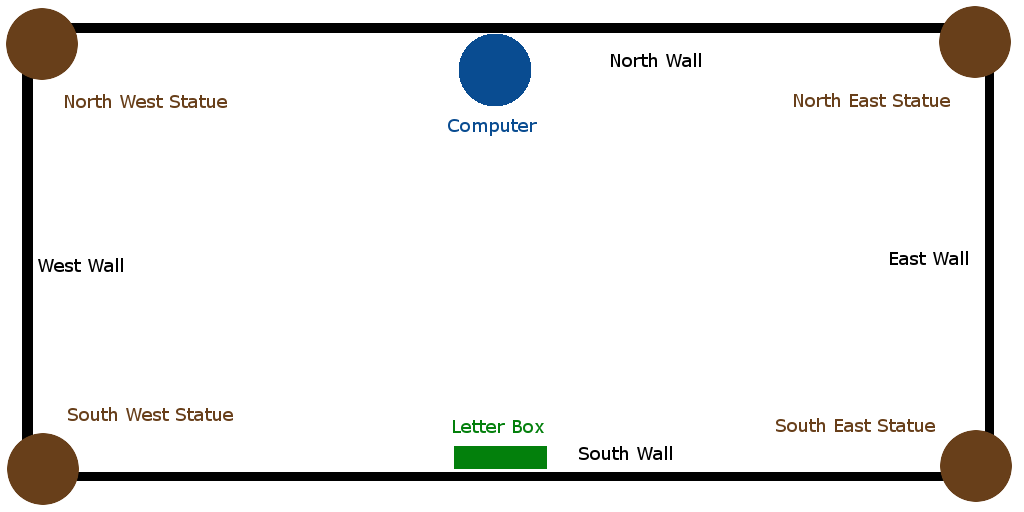
\includegraphics[width=6in]{RoomLayout1.png}
\end{figure}

\newpage
\section*{Letter 1}
After using the computer, a letter will fall through the letter box and you hear a click.
You first must read the letter by saying \textit{read letter}.

\epigraph{\textit{Better yourself, push your boundaries}}{Letter 1}

The solution to this puzzle is to push the north wall, you do this by interacting with it: \textit{interact with north wall}.
Once you've done this this, a second letter will fall through the letter box.
The room now looks like the diagram below once the wall is pushed.

\begin{figure}[htb]
	\centering
	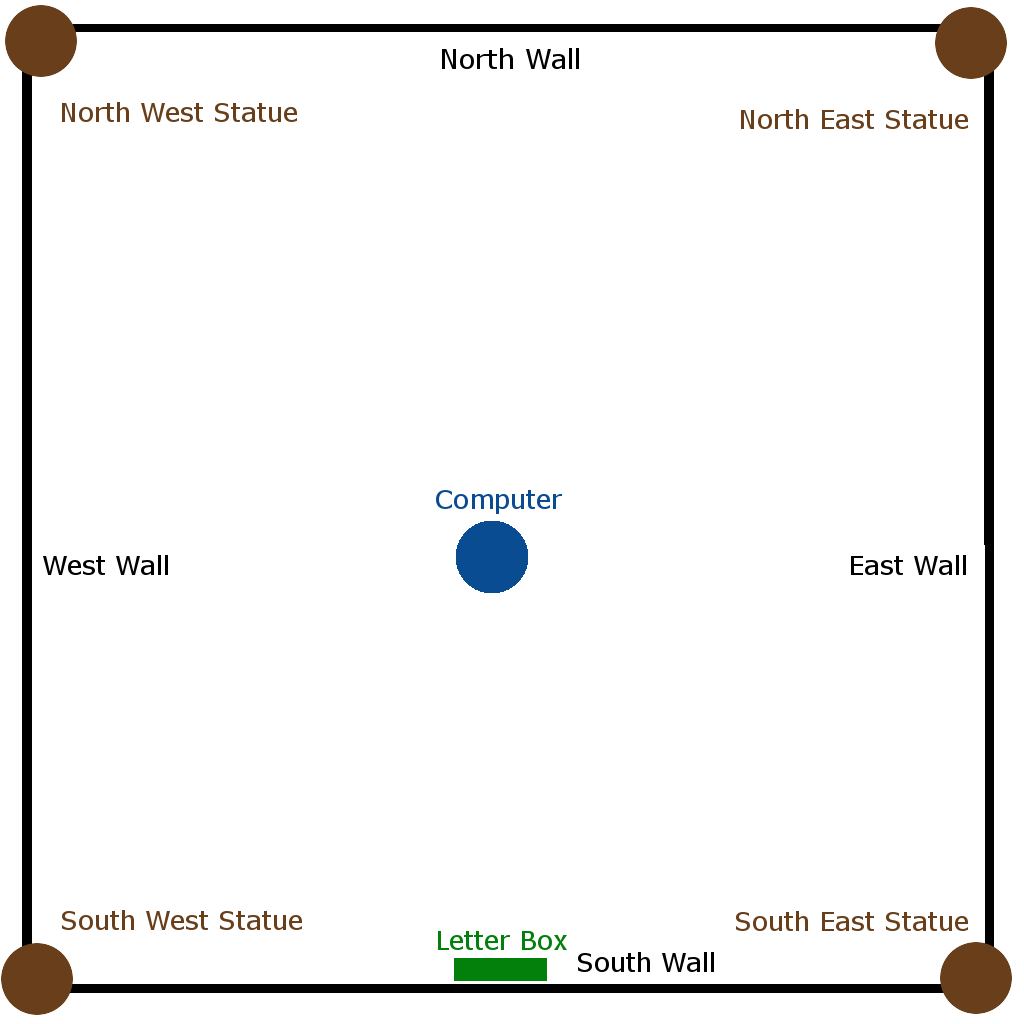
\includegraphics[width=3.5in]{RoomLayout2.png}
\end{figure}

\section*{Letter 2}
First you must read the second letter.

\epigraph{\textit{Prepare yourself, take a lap to clear your head}}{Letter 2}

The solution to this puzzle is to lap the entire room.
Although you can't give this command directly, you can lap the room by walking to each of the four statues in any order (provided it avoids moving across the room diagonally).
One such solution:

\begin{enumerate}
	\item \textit{walk to south west statue}
	\item \textit{walk to north west statue}
	\item \textit{walk to north east statue}
	\item \textit{walk to south east statue}
\end{enumerate}

\section*{Letter 3}
After completing a lap, another letter will fall through the letter box.
Once you read this letter, all the statues will open up and reveal computer terminals inside.

\epigraph{\textit{Frame yourself, act uncharacteristically for perspective}}{Letter 3}

\begin{figure}[htb]
	\centering
	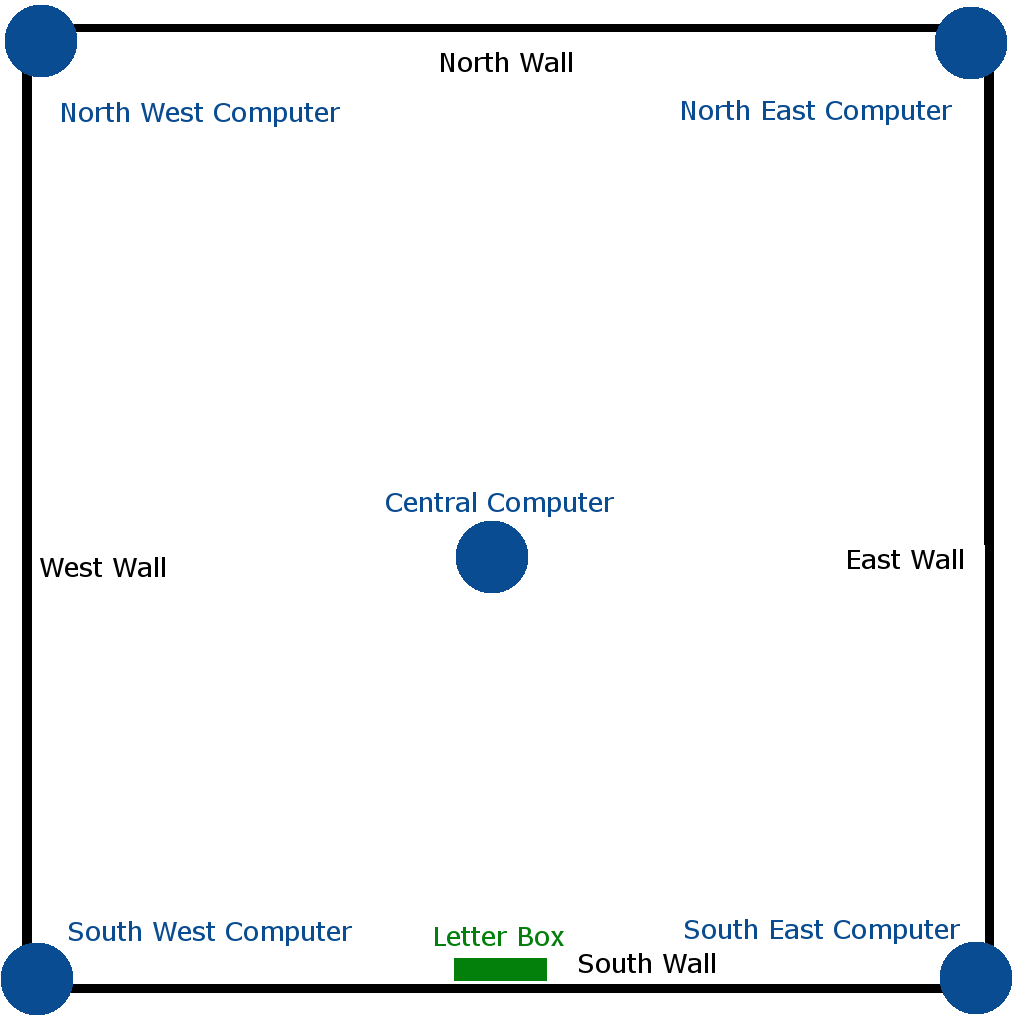
\includegraphics[width=3.5in]{RoomLayout3.png}
\end{figure}

Now that the statues have become computer terminals the room becomes the above diagram. You can now interact with the computers (for example: \textit{interact with north east computer}).
When you interact with the computers, each computer will display a sort of dream they aspire to achieve.
Each computer will then give you two options, one is an option of encouragement and the other is a cruel option.
To complete this puzzle you must be cruel to each of the four computers.
For the north west and south west terminals, option one is the cruel option.
For the north east and south east terminals, option two is the cruel option.
To select an option you just have to say \textit{option} followed by the number, for example \textit{option two}.

\newpage
\section*{Letter 4}
Once you've been cruel to each of the four computers, a forth letter will fall through the letter box.

\epigraph{\textit{Remove yourself, take a break from what you're doing}}{Letter 4}

For this puzzle you have to stop and start playing again.
To do this simply say \textit{stop}, and the game will end the session with your Alexa device.
Continue playing the game by saying \textit{Alexa play Puzzle Prison}, this will trigger the solution to the puzzle and one final letter will fall through the letter box.

\section*{The End}

To end the game, all you need to do is read the final letter.

\epigraph{\textit{Believe in yourself, it's time to go}}{The Final Letter}

To find out how the game ends, finish it yourself on your Alexa device.

\end{document}